\documentclass[a4paper,fleqn]{cas-sc}

% ----- Packages -----
% The cas-sc class (Elsevier CAS bundle) already loads graphicx, amsmath,
% amssymb, booktabs, xspace, xcolor, hyperref, and its own page geometry.
% We add only the packages it does not provide.
\usepackage[numbers]{natbib}
\usepackage{threeparttable}
\usepackage{float}
% cas-common.sty typesets every table caption in a \parbox whose width is
% \l_tbl_width_dim = \textwidth (its \__make_tbl_caption:nn). Inside a
% threeparttable, \hsize and \linewidth are still the provisional 160.9pt the
% package sets before the tabular width is known. A \textwidth parbox is
% emitted into a box less than a third as wide. TeX reports the resulting
% "Overfull \hbox (307.4pt too wide)", and the consequence is not cosmetic: the
% caption is set flush-right of the centred narrow box and its first line runs
% past the paper edge. Any caption long enough to wrap SILENTLY LOSES the
% words that fall off. Restore \hsize and \linewidth to the true text width
% (\columnwidth) for the duration of the caption, scoped to a group so the
% tabular's own width computation is untouched. This eliminates the overfull
% rather than hiding it, and every caption word is rendered.
\ExplSyntaxOn
\cs_if_exist:NT \__make_tbl_caption:nn
  {
    \cs_set_eq:NN \__cas_orig_make_tbl_caption:nn \__make_tbl_caption:nn
    \cs_set:Npn \__make_tbl_caption:nn #1#2
      { \group_begin: \hsize \columnwidth \linewidth \columnwidth
        \__cas_orig_make_tbl_caption:nn {#1} {#2} \group_end: }
  }
\ExplSyntaxOff
% Cross-document reference resolution for main-paper labels.
\usepackage{xr-hyper}
\externaldocument{paper}

% ----- Parameters -----
% ============================================================
% paper/params.tex
%
% Single source of truth for every numeric value cited in
% paper.tex. Two regions:
%
%   GENERATED REGION : rebuilt from regenerated CSV/parquet
%                      results under data/ by
%                      scripts/generate_params.py.
%                      Do NOT hand-edit.
%
%   MANUAL REGION    : fixed conventions (dataset names,
%                      axis bounds, hand-chosen documented
%                      thresholds). Hand-edited.
%
% Reproducibility: bash reproduce.sh re-runs every pipeline
% stage, regenerates this file's GENERATED region, then
% builds the paper. A diff in the produced PDF means a CSV
% cell drifted, and the responsible commit must be
% identified.
% ============================================================

% === BEGIN GENERATED REGION ===

% Design constants, read from the code that fixes them (subsec:methods, subsec:data_description, tab:settings)
\newcommand{\paperWindowDays}{60\xspace}
\newcommand{\paperStepDays}{20\xspace}
\newcommand{\paperPerQuintile}{300\xspace}
\newcommand{\minValidFractionPct}{80\%\xspace}
\newcommand{\minSectorSize}{20\xspace}
\newcommand{\minSectorStocksPerQuintile}{4\xspace}
\newcommand{\minSectorSizeLo}{15\xspace}
\newcommand{\minSectorSizeHi}{25\xspace}
\newcommand{\rollingMASteps}{6\xspace}
\newcommand{\blockBootDraws}{10{,}000\xspace}
\newcommand{\networkSizeNMin}{50\xspace}
\newcommand{\networkSizeNMax}{300\xspace}
\newcommand{\networkSizeNStep}{50\xspace}
\newcommand{\networkSizeWindowStride}{5\xspace}
\newcommand{\paperSampleStart}{2005\xspace}
\newcommand{\paperSampleEnd}{2025\xspace}
\newcommand{\blockBootLenHeadline}{6\xspace}

% Threshold scan grid (subsec:methods, tab:settings)
\newcommand{\rhoGridPoints}{200\xspace}
\newcommand{\rhoGridLo}{0.05\xspace}
\newcommand{\rhoGridHi}{0.90\xspace}
\newcommand{\splineMeshPoints}{2,000\xspace}

% Headline rho_c (tab:percolation, subsec:main_result)
\newcommand{\barRhoCQone}{0.524\xspace}
\newcommand{\barRhoCQtwo}{0.556\xspace}
\newcommand{\barRhoCQthree}{0.567\xspace}
\newcommand{\barRhoCQfour}{0.576\xspace}
\newcommand{\barRhoCQfive}{0.584\xspace}
\newcommand{\rhoCGapHeadline}{0.060\xspace}
\newcommand{\nWindowsHeadline}{257\xspace}
\newcommand{\medianStocksHeadlineQone}{279\xspace}
\newcommand{\rhoCStdHeadlineQone}{0.097\xspace}
\newcommand{\rhoCMinHeadlineQone}{0.398\xspace}
\newcommand{\rhoCMaxHeadlineQone}{0.879\xspace}
\newcommand{\medianStocksHeadlineQtwo}{290\xspace}
\newcommand{\rhoCStdHeadlineQtwo}{0.106\xspace}
\newcommand{\rhoCMinHeadlineQtwo}{0.397\xspace}
\newcommand{\rhoCMaxHeadlineQtwo}{0.886\xspace}
\newcommand{\medianStocksHeadlineQthree}{291\xspace}
\newcommand{\rhoCStdHeadlineQthree}{0.102\xspace}
\newcommand{\rhoCMinHeadlineQthree}{0.415\xspace}
\newcommand{\rhoCMaxHeadlineQthree}{0.874\xspace}
\newcommand{\medianStocksHeadlineQfour}{292\xspace}
\newcommand{\rhoCStdHeadlineQfour}{0.100\xspace}
\newcommand{\rhoCMinHeadlineQfour}{0.414\xspace}
\newcommand{\rhoCMaxHeadlineQfour}{0.891\xspace}
\newcommand{\medianStocksHeadlineQfive}{295\xspace}
\newcommand{\rhoCStdHeadlineQfive}{0.095\xspace}
\newcommand{\rhoCMinHeadlineQfive}{0.416\xspace}
\newcommand{\rhoCMaxHeadlineQfive}{0.880\xspace}

% KOSPI-only HAC t and block-bootstrap p (subsec:size_confounds, tab:robustness_summary)
\newcommand{\tHacKospiQoneQtwo}{5.01\xspace}
\newcommand{\pBlockBootKospiQoneQtwo}{< 10^{-4}\xspace}
\newcommand{\tHacKospiQtwoQthree}{0.17\xspace}
\newcommand{\pBlockBootKospiQtwoQthree}{= 0.50\xspace}
\newcommand{\tHacKospiQthreeQfour}{-0.87\xspace}
\newcommand{\pBlockBootKospiQthreeQfour}{= 0.75\xspace}
\newcommand{\tHacKospiQfourQfive}{5.46\xspace}
\newcommand{\pBlockBootKospiQfourQfive}{< 10^{-4}\xspace}

% Within-sector HAC t and block-bootstrap p (subsec:size_confounds, tab:robustness_summary)
\newcommand{\tHacWithinSectorQoneQtwo}{7.90\xspace}
\newcommand{\pBlockBootWithinSectorQoneQtwo}{< 10^{-4}\xspace}
\newcommand{\tHacWithinSectorQtwoQthree}{3.95\xspace}
\newcommand{\pBlockBootWithinSectorQtwoQthree}{= 3.0 \times 10^{-4}\xspace}
\newcommand{\tHacWithinSectorQthreeQfour}{0.93\xspace}
\newcommand{\pBlockBootWithinSectorQthreeQfour}{= 0.16\xspace}
\newcommand{\tHacWithinSectorQfourQfive}{1.87\xspace}
\newcommand{\pBlockBootWithinSectorQfourQfive}{= 0.04\xspace}

% Autocorrelation-robust headline significance (subsec:main_result, tab:pair_significance)
\newcommand{\tHacQoneQtwo}{9.6\xspace}
\newcommand{\pBlockBootQoneQtwo}{10^{-4}\xspace}
\newcommand{\tHacQtwoQthree}{3.1\xspace}
\newcommand{\pBlockBootQtwoQthree}{2.8 \times 10^{-3}\xspace}
\newcommand{\tHacQthreeQfour}{3.0\xspace}
\newcommand{\pBlockBootQthreeQfour}{2.7 \times 10^{-3}\xspace}
\newcommand{\tHacQfourQfive}{1.4\xspace}
\newcommand{\pBlockBootQfourQfive}{0.08\xspace}
\newcommand{\tHacQoneQfive}{6.8\xspace}
\newcommand{\fracWindowsAdjPairLo}{54\%\xspace}
\newcommand{\fracWindowsAdjPairHi}{84\%\xspace}
\newcommand{\pBlockBootQoneQfive}{10^{-4}\xspace}
\newcommand{\nwLagHeadline}{4\xspace}
\newcommand{\fracWindowsQoneLtQfiveKr}{83\%\xspace}

% Draw seeds and the spread of each step across the draws (subsec:methods, subsec:inference, tab:step_robustness)
\newcommand{\nDrawSeeds}{20\xspace}
\newcommand{\sdDrawKrQoneQtwo}{0.0029\xspace}
\newcommand{\sdDrawKrQtwoQthree}{0.0036\xspace}
\newcommand{\sdDrawKrQthreeQfour}{0.0037\xspace}
\newcommand{\sdDrawKrQfourQfive}{0.0037\xspace}
\newcommand{\sdDrawKrQoneQfive}{0.0026\xspace}
\newcommand{\sdDrawTwQoneQtwo}{0.0023\xspace}
\newcommand{\sdDrawTwQtwoQthree}{0.0024\xspace}
\newcommand{\sdDrawTwQthreeQfour}{0.0022\xspace}
\newcommand{\sdDrawTwQfourQfive}{0.0018\xspace}
\newcommand{\sdDrawTwQoneQfive}{0.0017\xspace}
\newcommand{\stepDrawSpreadRatioMin}{2.3\xspace}
\newcommand{\nDrawsRhoCAtGridEdge}{35\xspace}
\newcommand{\nDrawCellsHeadline}{25{,}700\xspace}

% Headline tests at longer bandwidths (subsec:inference, subsec:main_result, tab:step_robustness)
\newcommand{\bwShort}{12\xspace}
\newcommand{\bwLong}{24\xspace}
\newcommand{\tHacBwKrShortQoneQtwo}{8.1\xspace}
\newcommand{\pBlockBootBwKrShortQoneQtwo}{< 10^{-4}\xspace}
\newcommand{\tHacBwKrLongQoneQtwo}{7.5\xspace}
\newcommand{\pBlockBootBwKrLongQoneQtwo}{< 10^{-4}\xspace}
\newcommand{\tHacBwKrShortQtwoQthree}{2.4\xspace}
\newcommand{\pBlockBootBwKrShortQtwoQthree}{0.01\xspace}
\newcommand{\tHacBwKrLongQtwoQthree}{2.0\xspace}
\newcommand{\pBlockBootBwKrLongQtwoQthree}{0.045\xspace}
\newcommand{\tHacBwKrShortQthreeQfour}{2.4\xspace}
\newcommand{\pBlockBootBwKrShortQthreeQfour}{0.01\xspace}
\newcommand{\tHacBwKrLongQthreeQfour}{2.1\xspace}
\newcommand{\pBlockBootBwKrLongQthreeQfour}{0.03\xspace}
\newcommand{\tHacBwKrShortQfourQfive}{1.0\xspace}
\newcommand{\pBlockBootBwKrShortQfourQfive}{0.11\xspace}
\newcommand{\tHacBwKrLongQfourQfive}{0.9\xspace}
\newcommand{\pBlockBootBwKrLongQfourQfive}{0.12\xspace}
\newcommand{\tHacBwKrShortQoneQfive}{4.7\xspace}
\newcommand{\pBlockBootBwKrShortQoneQfive}{< 10^{-4}\xspace}
\newcommand{\tHacBwKrLongQoneQfive}{3.5\xspace}
\newcommand{\pBlockBootBwKrLongQoneQfive}{< 10^{-4}\xspace}
\newcommand{\tHacBwTwShortQoneQtwo}{9.4\xspace}
\newcommand{\pBlockBootBwTwShortQoneQtwo}{< 10^{-4}\xspace}
\newcommand{\tHacBwTwLongQoneQtwo}{9.1\xspace}
\newcommand{\pBlockBootBwTwLongQoneQtwo}{< 10^{-4}\xspace}
\newcommand{\tHacBwTwShortQtwoQthree}{7.0\xspace}
\newcommand{\pBlockBootBwTwShortQtwoQthree}{< 10^{-4}\xspace}
\newcommand{\tHacBwTwLongQtwoQthree}{7.6\xspace}
\newcommand{\pBlockBootBwTwLongQtwoQthree}{< 10^{-4}\xspace}
\newcommand{\tHacBwTwShortQthreeQfour}{7.3\xspace}
\newcommand{\pBlockBootBwTwShortQthreeQfour}{< 10^{-4}\xspace}
\newcommand{\tHacBwTwLongQthreeQfour}{7.2\xspace}
\newcommand{\pBlockBootBwTwLongQthreeQfour}{< 10^{-4}\xspace}
\newcommand{\tHacBwTwShortQfourQfive}{-0.6\xspace}
\newcommand{\pBlockBootBwTwShortQfourQfive}{0.75\xspace}
\newcommand{\tHacBwTwLongQfourQfive}{-0.6\xspace}
\newcommand{\pBlockBootBwTwLongQfourQfive}{0.76\xspace}
\newcommand{\tHacBwTwShortQoneQfive}{11.9\xspace}
\newcommand{\pBlockBootBwTwShortQoneQfive}{< 10^{-4}\xspace}
\newcommand{\tHacBwTwLongQoneQfive}{11.6\xspace}
\newcommand{\pBlockBootBwTwLongQoneQfive}{< 10^{-4}\xspace}

% rho_c from weekly returns on long windows (subsec:checks, subsec:main_result, tab:weekly_rho_c)
\newcommand{\detectPowerPct}{80\%\xspace}
\newcommand{\detectMultiplier}{2.49\xspace}
\newcommand{\wkWindowShort}{252\xspace}
\newcommand{\wkMedianWeeksShort}{54\xspace}
\newcommand{\wkLagShort}{13\xspace}
\newcommand{\wkWindowLong}{504\xspace}
\newcommand{\wkMedianWeeksLong}{107\xspace}
\newcommand{\wkLagLong}{26\xspace}
\newcommand{\wkKrShortDailyStepQoneQtwo}{+0.043\xspace}
\newcommand{\wkKrShortDailyTQoneQtwo}{6.9\xspace}
\newcommand{\wkKrShortDailyPQoneQtwo}{< 10^{-4}\xspace}
\newcommand{\wkKrShortWeeklyStepQoneQtwo}{+0.016\xspace}
\newcommand{\wkKrShortWeeklyTQoneQtwo}{4.7\xspace}
\newcommand{\wkKrShortWeeklyPQoneQtwo}{< 10^{-4}\xspace}
\newcommand{\wkKrShortDetectQoneQtwo}{0.009\xspace}
\newcommand{\wkKrShortDailyStepQtwoQthree}{+0.014\xspace}
\newcommand{\wkKrShortDailyTQtwoQthree}{2.9\xspace}
\newcommand{\wkKrShortDailyPQtwoQthree}{3.0 \times 10^{-4}\xspace}
\newcommand{\wkKrShortWeeklyStepQtwoQthree}{+0.004\xspace}
\newcommand{\wkKrShortWeeklyTQtwoQthree}{0.9\xspace}
\newcommand{\wkKrShortWeeklyPQtwoQthree}{0.13\xspace}
\newcommand{\wkKrShortDetectQtwoQthree}{0.011\xspace}
\newcommand{\wkKrShortDailyStepQthreeQfour}{+0.018\xspace}
\newcommand{\wkKrShortDailyTQthreeQfour}{4.0\xspace}
\newcommand{\wkKrShortDailyPQthreeQfour}{2.0 \times 10^{-4}\xspace}
\newcommand{\wkKrShortWeeklyStepQthreeQfour}{+0.008\xspace}
\newcommand{\wkKrShortWeeklyTQthreeQfour}{2.1\xspace}
\newcommand{\wkKrShortWeeklyPQthreeQfour}{0.03\xspace}
\newcommand{\wkKrShortDetectQthreeQfour}{0.009\xspace}
\newcommand{\wkKrShortDailyStepQfourQfive}{+0.040\xspace}
\newcommand{\wkKrShortDailyTQfourQfive}{2.6\xspace}
\newcommand{\wkKrShortDailyPQfourQfive}{3.0 \times 10^{-4}\xspace}
\newcommand{\wkKrShortWeeklyStepQfourQfive}{-0.000\xspace}
\newcommand{\wkKrShortWeeklyTQfourQfive}{-0.0\xspace}
\newcommand{\wkKrShortWeeklyPQfourQfive}{0.50\xspace}
\newcommand{\wkKrShortDetectQfourQfive}{0.021\xspace}
\newcommand{\wkKrShortDailyStepQoneQfive}{+0.115\xspace}
\newcommand{\wkKrShortDailyTQoneQfive}{4.8\xspace}
\newcommand{\wkKrShortDailyPQoneQfive}{< 10^{-4}\xspace}
\newcommand{\wkKrShortWeeklyStepQoneQfive}{+0.028\xspace}
\newcommand{\wkKrShortWeeklyTQoneQfive}{1.8\xspace}
\newcommand{\wkKrShortWeeklyPQoneQfive}{0.03\xspace}
\newcommand{\wkKrShortDetectQoneQfive}{0.039\xspace}
\newcommand{\wkKrLongDailyStepQoneQtwo}{+0.036\xspace}
\newcommand{\wkKrLongDailyTQoneQtwo}{4.4\xspace}
\newcommand{\wkKrLongDailyPQoneQtwo}{< 10^{-4}\xspace}
\newcommand{\wkKrLongWeeklyStepQoneQtwo}{+0.020\xspace}
\newcommand{\wkKrLongWeeklyTQoneQtwo}{3.1\xspace}
\newcommand{\wkKrLongWeeklyPQoneQtwo}{< 10^{-4}\xspace}
\newcommand{\wkKrLongDetectQoneQtwo}{0.016\xspace}
\newcommand{\wkKrLongDailyStepQtwoQthree}{+0.016\xspace}
\newcommand{\wkKrLongDailyTQtwoQthree}{3.0\xspace}
\newcommand{\wkKrLongDailyPQtwoQthree}{1.2 \times 10^{-3}\xspace}
\newcommand{\wkKrLongWeeklyStepQtwoQthree}{+0.010\xspace}
\newcommand{\wkKrLongWeeklyTQtwoQthree}{2.1\xspace}
\newcommand{\wkKrLongWeeklyPQtwoQthree}{0.01\xspace}
\newcommand{\wkKrLongDetectQtwoQthree}{0.012\xspace}
\newcommand{\wkKrLongDailyStepQthreeQfour}{+0.019\xspace}
\newcommand{\wkKrLongDailyTQthreeQfour}{3.4\xspace}
\newcommand{\wkKrLongDailyPQthreeQfour}{< 10^{-4}\xspace}
\newcommand{\wkKrLongWeeklyStepQthreeQfour}{+0.004\xspace}
\newcommand{\wkKrLongWeeklyTQthreeQfour}{0.6\xspace}
\newcommand{\wkKrLongWeeklyPQthreeQfour}{0.35\xspace}
\newcommand{\wkKrLongDetectQthreeQfour}{0.014\xspace}
\newcommand{\wkKrLongDailyStepQfourQfive}{+0.056\xspace}
\newcommand{\wkKrLongDailyTQfourQfive}{2.4\xspace}
\newcommand{\wkKrLongDailyPQfourQfive}{4.0 \times 10^{-4}\xspace}
\newcommand{\wkKrLongWeeklyStepQfourQfive}{+0.020\xspace}
\newcommand{\wkKrLongWeeklyTQfourQfive}{1.2\xspace}
\newcommand{\wkKrLongWeeklyPQfourQfive}{0.13\xspace}
\newcommand{\wkKrLongDetectQfourQfive}{0.041\xspace}
\newcommand{\wkKrLongDailyStepQoneQfive}{+0.126\xspace}
\newcommand{\wkKrLongDailyTQoneQfive}{3.3\xspace}
\newcommand{\wkKrLongDailyPQoneQfive}{< 10^{-4}\xspace}
\newcommand{\wkKrLongWeeklyStepQoneQfive}{+0.053\xspace}
\newcommand{\wkKrLongWeeklyTQoneQfive}{1.8\xspace}
\newcommand{\wkKrLongWeeklyPQoneQfive}{0.03\xspace}
\newcommand{\wkKrLongDetectQoneQfive}{0.073\xspace}
\newcommand{\wkTwShortDailyStepQoneQtwo}{+0.088\xspace}
\newcommand{\wkTwShortDailyTQoneQtwo}{14.2\xspace}
\newcommand{\wkTwShortDailyPQoneQtwo}{< 10^{-4}\xspace}
\newcommand{\wkTwShortWeeklyStepQoneQtwo}{+0.042\xspace}
\newcommand{\wkTwShortWeeklyTQoneQtwo}{8.5\xspace}
\newcommand{\wkTwShortWeeklyPQoneQtwo}{< 10^{-4}\xspace}
\newcommand{\wkTwShortDetectQoneQtwo}{0.012\xspace}
\newcommand{\wkTwShortDailyStepQtwoQthree}{+0.038\xspace}
\newcommand{\wkTwShortDailyTQtwoQthree}{8.6\xspace}
\newcommand{\wkTwShortDailyPQtwoQthree}{< 10^{-4}\xspace}
\newcommand{\wkTwShortWeeklyStepQtwoQthree}{+0.022\xspace}
\newcommand{\wkTwShortWeeklyTQtwoQthree}{5.1\xspace}
\newcommand{\wkTwShortWeeklyPQtwoQthree}{< 10^{-4}\xspace}
\newcommand{\wkTwShortDetectQtwoQthree}{0.011\xspace}
\newcommand{\wkTwShortDailyStepQthreeQfour}{+0.027\xspace}
\newcommand{\wkTwShortDailyTQthreeQfour}{4.6\xspace}
\newcommand{\wkTwShortDailyPQthreeQfour}{< 10^{-4}\xspace}
\newcommand{\wkTwShortWeeklyStepQthreeQfour}{+0.010\xspace}
\newcommand{\wkTwShortWeeklyTQthreeQfour}{2.3\xspace}
\newcommand{\wkTwShortWeeklyPQthreeQfour}{0.01\xspace}
\newcommand{\wkTwShortDetectQthreeQfour}{0.011\xspace}
\newcommand{\wkTwShortDailyStepQfourQfive}{+0.002\xspace}
\newcommand{\wkTwShortDailyTQfourQfive}{0.3\xspace}
\newcommand{\wkTwShortDailyPQfourQfive}{0.44\xspace}
\newcommand{\wkTwShortWeeklyStepQfourQfive}{-0.005\xspace}
\newcommand{\wkTwShortWeeklyTQfourQfive}{-0.8\xspace}
\newcommand{\wkTwShortWeeklyPQfourQfive}{0.80\xspace}
\newcommand{\wkTwShortDetectQfourQfive}{0.015\xspace}
\newcommand{\wkTwShortDailyStepQoneQfive}{+0.155\xspace}
\newcommand{\wkTwShortDailyTQoneQfive}{15.7\xspace}
\newcommand{\wkTwShortDailyPQoneQfive}{< 10^{-4}\xspace}
\newcommand{\wkTwShortWeeklyStepQoneQfive}{+0.069\xspace}
\newcommand{\wkTwShortWeeklyTQoneQfive}{9.0\xspace}
\newcommand{\wkTwShortWeeklyPQoneQfive}{< 10^{-4}\xspace}
\newcommand{\wkTwShortDetectQoneQfive}{0.019\xspace}
\newcommand{\wkTwLongDailyStepQoneQtwo}{+0.081\xspace}
\newcommand{\wkTwLongDailyTQoneQtwo}{13.0\xspace}
\newcommand{\wkTwLongDailyPQoneQtwo}{< 10^{-4}\xspace}
\newcommand{\wkTwLongWeeklyStepQoneQtwo}{+0.058\xspace}
\newcommand{\wkTwLongWeeklyTQoneQtwo}{8.6\xspace}
\newcommand{\wkTwLongWeeklyPQoneQtwo}{< 10^{-4}\xspace}
\newcommand{\wkTwLongDetectQoneQtwo}{0.017\xspace}
\newcommand{\wkTwLongDailyStepQtwoQthree}{+0.038\xspace}
\newcommand{\wkTwLongDailyTQtwoQthree}{5.9\xspace}
\newcommand{\wkTwLongDailyPQtwoQthree}{< 10^{-4}\xspace}
\newcommand{\wkTwLongWeeklyStepQtwoQthree}{+0.017\xspace}
\newcommand{\wkTwLongWeeklyTQtwoQthree}{3.1\xspace}
\newcommand{\wkTwLongWeeklyPQtwoQthree}{5.0 \times 10^{-4}\xspace}
\newcommand{\wkTwLongDetectQtwoQthree}{0.014\xspace}
\newcommand{\wkTwLongDailyStepQthreeQfour}{+0.031\xspace}
\newcommand{\wkTwLongDailyTQthreeQfour}{4.4\xspace}
\newcommand{\wkTwLongDailyPQthreeQfour}{< 10^{-4}\xspace}
\newcommand{\wkTwLongWeeklyStepQthreeQfour}{+0.015\xspace}
\newcommand{\wkTwLongWeeklyTQthreeQfour}{2.9\xspace}
\newcommand{\wkTwLongWeeklyPQthreeQfour}{3.0 \times 10^{-4}\xspace}
\newcommand{\wkTwLongDetectQthreeQfour}{0.013\xspace}
\newcommand{\wkTwLongDailyStepQfourQfive}{+0.005\xspace}
\newcommand{\wkTwLongDailyTQfourQfive}{0.8\xspace}
\newcommand{\wkTwLongDailyPQfourQfive}{0.32\xspace}
\newcommand{\wkTwLongWeeklyStepQfourQfive}{-0.010\xspace}
\newcommand{\wkTwLongWeeklyTQfourQfive}{-1.3\xspace}
\newcommand{\wkTwLongWeeklyPQfourQfive}{0.95\xspace}
\newcommand{\wkTwLongDetectQfourQfive}{0.019\xspace}
\newcommand{\wkTwLongDailyStepQoneQfive}{+0.156\xspace}
\newcommand{\wkTwLongDailyTQoneQfive}{15.3\xspace}
\newcommand{\wkTwLongDailyPQoneQfive}{< 10^{-4}\xspace}
\newcommand{\wkTwLongWeeklyStepQoneQfive}{+0.080\xspace}
\newcommand{\wkTwLongWeeklyTQoneQfive}{6.9\xspace}
\newcommand{\wkTwLongWeeklyPQoneQfive}{< 10^{-4}\xspace}
\newcommand{\wkTwLongDetectQoneQfive}{0.029\xspace}

% KOSPI-only resolution of the interior steps (subsec:main_result)
\newcommand{\kospiDetectMin}{0.013\xspace}

% Steps under the estimation settings (subsec:researcher_choices, tab:setting_steps)
\newcommand{\tHacWthirtyQoneQtwo}{10.2\xspace}
\newcommand{\pBootWthirtyQoneQtwo}{< 10^{-4}\xspace}
\newcommand{\tHacWthirtyQtwoQthree}{3.7\xspace}
\newcommand{\pBootWthirtyQtwoQthree}{< 10^{-4}\xspace}
\newcommand{\tHacWthirtyQthreeQfour}{0.4\xspace}
\newcommand{\pBootWthirtyQthreeQfour}{0.45\xspace}
\newcommand{\detectWthirtyQthreeQfour}{0.007\xspace}
\newcommand{\tHacWthirtyQfourQfive}{0.8\xspace}
\newcommand{\pBootWthirtyQfourQfive}{0.20\xspace}
\newcommand{\tHacWthirtyQoneQfive}{6.2\xspace}
\newcommand{\pBootWthirtyQoneQfive}{< 10^{-4}\xspace}
\newcommand{\tHacWhundredtwentyQoneQtwo}{7.2\xspace}
\newcommand{\pBootWhundredtwentyQoneQtwo}{< 10^{-4}\xspace}
\newcommand{\tHacWhundredtwentyQtwoQthree}{3.8\xspace}
\newcommand{\pBootWhundredtwentyQtwoQthree}{< 10^{-4}\xspace}
\newcommand{\tHacWhundredtwentyQthreeQfour}{4.2\xspace}
\newcommand{\pBootWhundredtwentyQthreeQfour}{< 10^{-4}\xspace}
\newcommand{\tHacWhundredtwentyQfourQfive}{2.7\xspace}
\newcommand{\pBootWhundredtwentyQfourQfive}{1.4 \times 10^{-3}\xspace}
\newcommand{\tHacWhundredtwentyQoneQfive}{7.0\xspace}
\newcommand{\pBootWhundredtwentyQoneQfive}{< 10^{-4}\xspace}
\newcommand{\tHacWtwofiftyQoneQtwo}{6.9\xspace}
\newcommand{\pBootWtwofiftyQoneQtwo}{< 10^{-4}\xspace}
\newcommand{\tHacWtwofiftyQtwoQthree}{2.9\xspace}
\newcommand{\pBootWtwofiftyQtwoQthree}{3.0 \times 10^{-4}\xspace}
\newcommand{\tHacWtwofiftyQthreeQfour}{4.0\xspace}
\newcommand{\pBootWtwofiftyQthreeQfour}{2.0 \times 10^{-4}\xspace}
\newcommand{\tHacWtwofiftyQfourQfive}{2.6\xspace}
\newcommand{\pBootWtwofiftyQfourQfive}{3.0 \times 10^{-4}\xspace}
\newcommand{\tHacWtwofiftyQoneQfive}{4.8\xspace}
\newcommand{\pBootWtwofiftyQoneQfive}{< 10^{-4}\xspace}
\newcommand{\tHacObsReqLoQoneQtwo}{9.6\xspace}
\newcommand{\pBootObsReqLoQoneQtwo}{< 10^{-4}\xspace}
\newcommand{\tHacObsReqLoQtwoQthree}{3.0\xspace}
\newcommand{\pBootObsReqLoQtwoQthree}{3.7 \times 10^{-3}\xspace}
\newcommand{\tHacObsReqLoQthreeQfour}{3.1\xspace}
\newcommand{\pBootObsReqLoQthreeQfour}{1.9 \times 10^{-3}\xspace}
\newcommand{\tHacObsReqLoQfourQfive}{1.3\xspace}
\newcommand{\pBootObsReqLoQfourQfive}{0.09\xspace}
\newcommand{\tHacObsReqLoQoneQfive}{7.0\xspace}
\newcommand{\pBootObsReqLoQoneQfive}{< 10^{-4}\xspace}
\newcommand{\tHacObsReqHiQoneQtwo}{9.8\xspace}
\newcommand{\pBootObsReqHiQoneQtwo}{< 10^{-4}\xspace}
\newcommand{\tHacObsReqHiQtwoQthree}{3.3\xspace}
\newcommand{\pBootObsReqHiQtwoQthree}{1.8 \times 10^{-3}\xspace}
\newcommand{\tHacObsReqHiQthreeQfour}{2.8\xspace}
\newcommand{\pBootObsReqHiQthreeQfour}{6.2 \times 10^{-3}\xspace}
\newcommand{\tHacObsReqHiQfourQfive}{1.4\xspace}
\newcommand{\pBootObsReqHiQfourQfive}{0.07\xspace}
\newcommand{\tHacObsReqHiQoneQfive}{6.8\xspace}
\newcommand{\pBootObsReqHiQoneQfive}{< 10^{-4}\xspace}
\newcommand{\detectChiQthreeQfour}{0.008\xspace}
\newcommand{\detectWithinSectorQthreeQfour}{0.0094\xspace}
\newcommand{\rhoCStepHeadlineQthreeQfourFine}{0.0089\xspace}

% rho_c / mean |rho| coupling (subsec:threshold_vs_mean)
\newcommand{\meanCorrSpearman}{0.95\xspace}
\newcommand{\rhoCResidGapPctOfRaw}{33\%\xspace}
\newcommand{\rhoCResidGapPctOfRawDegLo}{27\%\xspace}
\newcommand{\rhoCResidGapPctOfRawDegHi}{53\%\xspace}
\newcommand{\tHacMeanCorrResidQoneQfive}{5.4\xspace}
\newcommand{\meanAbsCorrQone}{0.182\xspace}
\newcommand{\meanAbsCorrQtwo}{0.198\xspace}
\newcommand{\meanAbsCorrQthree}{0.204\xspace}
\newcommand{\meanAbsCorrQfour}{0.206\xspace}
\newcommand{\meanAbsCorrQfive}{0.207\xspace}
\newcommand{\tHacMeanCorrQoneQfive}{3.7\xspace}

% rho_c over the network size (subsec:threshold_vs_mean)
\newcommand{\rhoCSlopeSqrtLogN}{0.167\xspace}

% Korean universe (subsec:data_description)
\newcommand{\nStocksKoreaTotal}{3{,}293\xspace}
\newcommand{\nDaysKoreaTotal}{5{,}182\xspace}

% Korean panel coverage (subsec:data_description)
\newcommand{\krPanelStart}{2005-01-03\xspace}
\newcommand{\krPanelEnd}{2025-12-30\xspace}

% Taiwan universe (subsec:data_description)
\newcommand{\nStocksTaiwanTotal}{2{,}066\xspace}
\newcommand{\nDaysTaiwanTotal}{5{,}166\xspace}

% Taiwan panel coverage (subsec:data_description)
\newcommand{\twPanelStart}{2005-01-03\xspace}
\newcommand{\twPanelEnd}{2025-12-31\xspace}

% Susceptibility-peak rho_c (tab:percolation, subsec:main_result, subsec:researcher_choices)
\newcommand{\barRhoCChiQone}{0.583\xspace}
\newcommand{\barRhoCChiQtwo}{0.614\xspace}
\newcommand{\barRhoCChiQthree}{0.623\xspace}
\newcommand{\barRhoCChiQfour}{0.623\xspace}
\newcommand{\barRhoCChiQfive}{0.631\xspace}
\newcommand{\rhoCGapChi}{0.047\xspace}
\newcommand{\rhoCChiOffsetMin}{0.047\xspace}
\newcommand{\rhoCChiOffsetMax}{0.059\xspace}
\newcommand{\tHacChiQthreeQfour}{0.03\xspace}
\newcommand{\tHacChiQfourQfive}{0.97\xspace}

% KOSPI-only robustness (subsec:checks, subsec:main_result, tab:robustness_summary)
\newcommand{\rhoCGapKospi}{0.068\xspace}

% Panel construction (tab:settings)
\newcommand{\noTradeShareKr}{2.2\%\xspace}
\newcommand{\noTradeShareTw}{0.8\%\xspace}

% Within-sector robustness (subsec:main_result, subsec:size_confounds, tab:robustness_contrast)
\newcommand{\rhoCGapWithinSector}{0.048\xspace}
\newcommand{\rhoCGapWithinSectorPctOfHeadline}{81\%\xspace}
\newcommand{\rhoCGapWithinSectorFloorMin}{0.048\xspace}
\newcommand{\rhoCGapWithinSectorFloorMax}{0.050\xspace}

% RMT-cleaned rho_c (subsec:main_result, tab:robustness_summary)
\newcommand{\barRhoCRmtQone}{0.497\xspace}
\newcommand{\barRhoCRmtQtwo}{0.533\xspace}
\newcommand{\barRhoCRmtQthree}{0.543\xspace}
\newcommand{\barRhoCRmtQfour}{0.553\xspace}
\newcommand{\barRhoCRmtQfive}{0.565\xspace}
\newcommand{\rhoCGapRmt}{0.068\xspace}

% Subperiod stability (subsec:subperiod, tab:subperiod)
\newcommand{\tHacEndpointEarly}{8.3\xspace}
\newcommand{\tHacEndpointLate}{3.0\xspace}
\newcommand{\tHacEndpointEarlyTw}{10.2\xspace}
\newcommand{\tHacEndpointLateTw}{12.9\xspace}
\newcommand{\rhoCGapEndpointEarly}{+0.097\xspace}
\newcommand{\rhoCGapEndpointLate}{+0.023\xspace}
\newcommand{\rhoCGapEndpointEarlyTw}{+0.120\xspace}
\newcommand{\rhoCGapEndpointLateTw}{+0.104\xspace}
\newcommand{\pBootEndpointLate}{2.1 \times 10^{-3}\xspace}
\newcommand{\fracWindowsLateQoneLtQfive}{71\%\xspace}
\newcommand{\rhoCGapLateShareOfEarlyPct}{23\%\xspace}
\newcommand{\rhoCGapLateShareOfEarlyTwPct}{86\%\xspace}
\newcommand{\krUnresolvedBlock}{2015--2019\xspace}
\newcommand{\yearBlockA}{2005--2009\xspace}
\newcommand{\tHacYearBlockKrA}{8.2\xspace}
\newcommand{\tHacYearBlockTwA}{7.9\xspace}
\newcommand{\yearBlockB}{2010--2014\xspace}
\newcommand{\tHacYearBlockKrB}{5.8\xspace}
\newcommand{\tHacYearBlockTwB}{8.4\xspace}
\newcommand{\yearBlockC}{2015--2019\xspace}
\newcommand{\tHacYearBlockKrC}{1.6\xspace}
\newcommand{\tHacYearBlockTwC}{11.6\xspace}
\newcommand{\yearBlockD}{2020--2025\xspace}
\newcommand{\tHacYearBlockKrD}{2.8\xspace}
\newcommand{\tHacYearBlockTwD}{10.5\xspace}

% Second-half subsample (subsec:subperiod)
\newcommand{\nWindowsSecondHalf}{129\xspace}
\newcommand{\secondHalfStart}{2015-07-22\xspace}
\newcommand{\tHacSecondHalfQoneQtwo}{6.3\xspace}
\newcommand{\rhoCStepSecondHalfQoneQtwo}{+0.030\xspace}
\newcommand{\tHacSecondHalfQtwoQthree}{-0.1\xspace}
\newcommand{\tHacSecondHalfQthreeQfour}{1.2\xspace}
\newcommand{\tHacSecondHalfQfourQfive}{-2.2\xspace}
\newcommand{\rhoCStepSecondHalfQfourQfive}{-0.012\xspace}
\newcommand{\rhoCSecondHalfInteriorSpan}{0.005\xspace}

% Taiwan re-run (subsec:taiwan, tab:taiwan_rerun, subsec:threshold_vs_mean)
\newcommand{\medianStocksTwQone}{262\xspace}
\newcommand{\barRhoCTwQone}{0.521\xspace}
\newcommand{\barRhoCChiTwQone}{0.578\xspace}
\newcommand{\medianStocksTwQtwo}{285\xspace}
\newcommand{\barRhoCTwQtwo}{0.577\xspace}
\newcommand{\barRhoCChiTwQtwo}{0.641\xspace}
\newcommand{\medianStocksTwQthree}{290\xspace}
\newcommand{\barRhoCTwQthree}{0.609\xspace}
\newcommand{\barRhoCChiTwQthree}{0.657\xspace}
\newcommand{\medianStocksTwQfour}{292\xspace}
\newcommand{\barRhoCTwQfour}{0.635\xspace}
\newcommand{\barRhoCChiTwQfour}{0.671\xspace}
\newcommand{\medianStocksTwQfive}{296\xspace}
\newcommand{\barRhoCTwQfive}{0.633\xspace}
\newcommand{\barRhoCChiTwQfive}{0.666\xspace}
\newcommand{\rhoCGapTw}{0.112\xspace}
\newcommand{\rhoCGapTwQFiveMinusQFour}{-0.002\xspace}
\newcommand{\nWindowsTw}{256\xspace}
\newcommand{\rhoCGapTwNImplied}{0.006\xspace}
\newcommand{\rhoCGapTwNImpliedPct}{5\%\xspace}
\newcommand{\rhoCGapKrNImplied}{0.003\xspace}
\newcommand{\rhoCGapKrNImpliedPct}{5\%\xspace}
\newcommand{\fracWindowsQoneLtQfiveTw}{96\%\xspace}
\newcommand{\tHacTwQoneQtwo}{11.1\xspace}
\newcommand{\pBlockBootTwQoneQtwo}{10^{-4}\xspace}
\newcommand{\tHacTwQtwoQthree}{7.3\xspace}
\newcommand{\pBlockBootTwQtwoQthree}{10^{-4}\xspace}
\newcommand{\tHacTwQthreeQfour}{8.4\xspace}
\newcommand{\pBlockBootTwQthreeQfour}{10^{-4}\xspace}
\newcommand{\tHacTwQfourQfive}{-0.7\xspace}
\newcommand{\pBlockBootTwQfourQfive}{0.77\xspace}
\newcommand{\tHacTwQoneQfive}{15.6\xspace}
\newcommand{\pBlockBootTwQoneQfive}{10^{-4}\xspace}
\newcommand{\tHacTwChiQoneQfive}{11.9\xspace}
\newcommand{\tHacTwChiStepMin}{4.9\xspace}
\newcommand{\tHacTwChiStepMax}{15.4\xspace}
\newcommand{\tHacTwChiQfourQfive}{-1.2\xspace}

% Shuffled-returns null (subsec:checks, subsec:main_result, tab:robustness_summary)
\newcommand{\shuffNullRhoCQone}{0.376\xspace}
\newcommand{\shuffNullRhoCQtwo}{0.376\xspace}
\newcommand{\shuffNullRhoCQthree}{0.374\xspace}
\newcommand{\shuffNullRhoCQfour}{0.371\xspace}
\newcommand{\shuffNullRhoCQfive}{0.368\xspace}
\newcommand{\shuffNullGapQFiveMinusQone}{-0.008\xspace}
\newcommand{\nShuffleSeeds}{20\xspace}
\newcommand{\shuffNullSeedSdMax}{0.0004\xspace}

% Per-quintile excess kurtosis of daily returns (subsec:null_robustness)
\newcommand{\excessKurtQone}{3.8\xspace}
\newcommand{\excessKurtQfive}{2.0\xspace}

% Window-length sensitivity (subsec:checks, subsec:main_result, tab:robustness_summary)
\newcommand{\barRhoCWthirtyQone}{0.630\xspace}
\newcommand{\barRhoCWthirtyQtwo}{0.654\xspace}
\newcommand{\barRhoCWthirtyQthree}{0.664\xspace}
\newcommand{\barRhoCWthirtyQfour}{0.665\xspace}
\newcommand{\barRhoCWthirtyQfive}{0.668\xspace}
\newcommand{\barRhoCWhundredtwentyQone}{0.443\xspace}
\newcommand{\barRhoCWhundredtwentyQtwo}{0.480\xspace}
\newcommand{\barRhoCWhundredtwentyQthree}{0.493\xspace}
\newcommand{\barRhoCWhundredtwentyQfour}{0.509\xspace}
\newcommand{\barRhoCWhundredtwentyQfive}{0.531\xspace}
\newcommand{\barRhoCWtwofiftyQone}{0.380\xspace}
\newcommand{\barRhoCWtwofiftyQtwo}{0.423\xspace}
\newcommand{\barRhoCWtwofiftyQthree}{0.437\xspace}
\newcommand{\barRhoCWtwofiftyQfour}{0.455\xspace}
\newcommand{\barRhoCWtwofiftyQfive}{0.495\xspace}
\newcommand{\windowDaysWthirty}{30\xspace}
\newcommand{\rhoCGapWthirty}{0.038\xspace}
\newcommand{\nWindowsWthirty}{258\xspace}
\newcommand{\windowDaysWhundredtwenty}{120\xspace}
\newcommand{\rhoCGapWhundredtwenty}{0.088\xspace}
\newcommand{\nWindowsWhundredtwenty}{254\xspace}
\newcommand{\windowDaysWtwofifty}{252\xspace}
\newcommand{\rhoCGapWtwofifty}{0.115\xspace}
\newcommand{\nWindowsWtwofifty}{247\xspace}

% Observation-requirement sensitivity (subsec:checks, subsec:researcher_choices, tab:robustness_summary)
\newcommand{\minValidFractionLoPct}{70\%\xspace}
\newcommand{\minValidFractionHiPct}{90\%\xspace}
\newcommand{\barRhoCObsReqLoQone}{0.525\xspace}
\newcommand{\barRhoCObsReqLoQtwo}{0.557\xspace}
\newcommand{\barRhoCObsReqLoQthree}{0.566\xspace}
\newcommand{\barRhoCObsReqLoQfour}{0.576\xspace}
\newcommand{\barRhoCObsReqLoQfive}{0.584\xspace}
\newcommand{\rhoCGapObsReqLo}{0.058\xspace}
\newcommand{\barRhoCObsReqHiQone}{0.524\xspace}
\newcommand{\barRhoCObsReqHiQtwo}{0.556\xspace}
\newcommand{\barRhoCObsReqHiQthree}{0.567\xspace}
\newcommand{\barRhoCObsReqHiQfour}{0.576\xspace}
\newcommand{\barRhoCObsReqHiQfive}{0.584\xspace}
\newcommand{\rhoCGapObsReqHi}{0.060\xspace}

% Marchenko-Pastur noise band (subsec:checks)
\newcommand{\mpLambdaMinus}{1.53\xspace}
\newcommand{\mpLambdaPlus}{10.47\xspace}

% Residualization: adjacent steps and endpoint of rho_c (subsec:residuals, tab:residual_steps)
\newcommand{\rhoCStepHeadlineQoneQtwo}{+0.032\xspace}
\newcommand{\rhoCStepHeadlineQtwoQthree}{+0.010\xspace}
\newcommand{\rhoCStepHeadlineQthreeQfour}{+0.009\xspace}
\newcommand{\rhoCStepHeadlineQfourQfive}{+0.008\xspace}
\newcommand{\rhoCRiseQoneQfourHeadline}{+0.052\xspace}
\newcommand{\rhoCStepMktResidQoneQtwo}{+0.014\xspace}
\newcommand{\tHacMktResidQoneQtwo}{5.7\xspace}
\newcommand{\rhoCStepMktResidQtwoQthree}{-0.001\xspace}
\newcommand{\tHacMktResidQtwoQthree}{-0.4\xspace}
\newcommand{\rhoCStepMktResidQthreeQfour}{-0.009\xspace}
\newcommand{\tHacMktResidQthreeQfour}{-4.1\xspace}
\newcommand{\rhoCStepMktResidQfourQfive}{+0.001\xspace}
\newcommand{\tHacMktResidQfourQfive}{0.5\xspace}
\newcommand{\rhoCGapMktResid}{+0.006\xspace}
\newcommand{\tHacMktResidQoneQfive}{1.3\xspace}
\newcommand{\rhoCStepMktResidEwQoneQtwo}{+0.004\xspace}
\newcommand{\tHacMktResidEwQoneQtwo}{3.2\xspace}
\newcommand{\rhoCStepMktResidEwQtwoQthree}{-0.001\xspace}
\newcommand{\tHacMktResidEwQtwoQthree}{-0.5\xspace}
\newcommand{\rhoCStepMktResidEwQthreeQfour}{+0.006\xspace}
\newcommand{\tHacMktResidEwQthreeQfour}{5.2\xspace}
\newcommand{\rhoCStepMktResidEwQfourQfive}{+0.049\xspace}
\newcommand{\tHacMktResidEwQfourQfive}{16.6\xspace}
\newcommand{\rhoCGapMktResidEw}{+0.058\xspace}
\newcommand{\tHacMktResidEwQoneQfive}{17.7\xspace}
\newcommand{\rhoCStepMktSecResidQoneQtwo}{+0.003\xspace}
\newcommand{\tHacMktSecResidQoneQtwo}{1.8\xspace}
\newcommand{\rhoCStepMktSecResidQtwoQthree}{-0.005\xspace}
\newcommand{\tHacMktSecResidQtwoQthree}{-3.4\xspace}
\newcommand{\rhoCStepMktSecResidQthreeQfour}{-0.010\xspace}
\newcommand{\tHacMktSecResidQthreeQfour}{-4.9\xspace}
\newcommand{\rhoCStepMktSecResidQfourQfive}{+0.001\xspace}
\newcommand{\tHacMktSecResidQfourQfive}{0.4\xspace}
\newcommand{\rhoCGapMktSecResid}{-0.011\xspace}
\newcommand{\tHacMktSecResidQoneQfive}{-3.8\xspace}
\newcommand{\rhoCStepMktSecResidEwQoneQtwo}{-0.000\xspace}
\newcommand{\tHacMktSecResidEwQoneQtwo}{-0.4\xspace}
\newcommand{\rhoCStepMktSecResidEwQtwoQthree}{-0.002\xspace}
\newcommand{\tHacMktSecResidEwQtwoQthree}{-2.8\xspace}
\newcommand{\rhoCStepMktSecResidEwQthreeQfour}{-0.002\xspace}
\newcommand{\tHacMktSecResidEwQthreeQfour}{-2.5\xspace}
\newcommand{\rhoCStepMktSecResidEwQfourQfive}{+0.026\xspace}
\newcommand{\tHacMktSecResidEwQfourQfive}{18.5\xspace}
\newcommand{\rhoCGapMktSecResidEw}{+0.021\xspace}
\newcommand{\tHacMktSecResidEwQoneQfive}{10.0\xspace}
\newcommand{\rhoCRiseQoneQfourResidMin}{-0.012\xspace}
\newcommand{\rhoCRiseQoneQfourResidMax}{+0.010\xspace}

% KOSPI-only robustness (subsec:checks, subsec:main_result, tab:robustness_summary)
\newcommand{\barRhoCKospiQone}{0.514\xspace}
\newcommand{\medianStocksKospiQone}{145\xspace}
\newcommand{\barRhoCKospiQtwo}{0.539\xspace}
\newcommand{\barRhoCKospiQthree}{0.540\xspace}
\newcommand{\barRhoCKospiQfour}{0.535\xspace}
\newcommand{\barRhoCKospiQfive}{0.582\xspace}
\newcommand{\medianStocksKospiQfive}{149\xspace}
\newcommand{\nWindowsKospi}{257\xspace}
\newcommand{\nKospiTickers}{1{,}020\xspace}

% Within-sector per-quintile (subsec:size_confounds, tab:robustness_summary)
\newcommand{\barRhoCWithinSectorQone}{0.529\xspace}
\newcommand{\medianStocksWithinSectorQone}{281\xspace}
\newcommand{\barRhoCWithinSectorQtwo}{0.554\xspace}
\newcommand{\barRhoCWithinSectorQthree}{0.566\xspace}
\newcommand{\barRhoCWithinSectorQfour}{0.569\xspace}
\newcommand{\barRhoCWithinSectorQfive}{0.577\xspace}
\newcommand{\medianStocksWithinSectorQfive}{294\xspace}
\newcommand{\nWindowsWithinSector}{257\xspace}

% DGP eq:toy_threshold/eq:toy_closed_form verification (si:eq9_verification)
\newcommand{\rhoCDgpSimDeltaA}{0.668\xspace}
\newcommand{\rhoCDgpSimDegOneDeltaA}{0.667\xspace}
\newcommand{\rhoCDgpClosedDeltaA}{0.811\xspace}
\newcommand{\rhoCDgpSimDeltaB}{0.626\xspace}
\newcommand{\rhoCDgpSimDegOneDeltaB}{0.620\xspace}
\newcommand{\rhoCDgpClosedDeltaB}{0.743\xspace}
\newcommand{\rhoCDgpSimDeltaC}{0.575\xspace}
\newcommand{\rhoCDgpSimDegOneDeltaC}{0.571\xspace}
\newcommand{\rhoCDgpClosedDeltaC}{0.667\xspace}
\newcommand{\rhoCDgpSimDeltaD}{0.537\xspace}
\newcommand{\rhoCDgpSimDegOneDeltaD}{0.534\xspace}
\newcommand{\rhoCDgpClosedDeltaD}{0.608\xspace}
\newcommand{\rhoCDgpSimDeltaE}{0.493\xspace}
\newcommand{\rhoCDgpSimDegOneDeltaE}{0.484\xspace}
\newcommand{\rhoCDgpClosedDeltaE}{0.528\xspace}
\newcommand{\rhoCDgpSimSectorDeltaA}{0.715\xspace}
\newcommand{\rhoCDgpSimSectorDegOneDeltaA}{0.722\xspace}
\newcommand{\rhoCDgpClosedSectorDeltaA}{0.901\xspace}
\newcommand{\rhoCDgpSimSectorDeltaB}{0.640\xspace}
\newcommand{\rhoCDgpSimSectorDegOneDeltaB}{0.642\xspace}
\newcommand{\rhoCDgpClosedSectorDeltaB}{0.780\xspace}
\newcommand{\rhoCDgpSimSectorDeltaC}{0.582\xspace}
\newcommand{\rhoCDgpSimSectorDegOneDeltaC}{0.581\xspace}
\newcommand{\rhoCDgpClosedSectorDeltaC}{0.687\xspace}
\newcommand{\rhoCDgpSimSectorDeltaD}{0.542\xspace}
\newcommand{\rhoCDgpSimSectorDegOneDeltaD}{0.535\xspace}
\newcommand{\rhoCDgpClosedSectorDeltaD}{0.610\xspace}
\newcommand{\rhoCDgpSimSectorDeltaE}{0.490\xspace}
\newcommand{\rhoCDgpSimSectorDegOneDeltaE}{0.483\xspace}
\newcommand{\rhoCDgpClosedSectorDeltaE}{0.526\xspace}
\newcommand{\dgpEqEightMaxGap}{0.010\xspace}
\newcommand{\nDgpEqEightCells}{10\xspace}
\newcommand{\dgpDegOneMinFall}{0.037\xspace}
\newcommand{\dgpEqNineOvershootLo}{0.035\xspace}
\newcommand{\dgpEqNineOvershootHi}{0.186\xspace}

% DGP simulation constants (si:dgp_validation)
\newcommand{\dgpSigmaF}{0.007\xspace}
\newcommand{\dgpSigmaU}{0.02\xspace}
\newcommand{\dgpSigmaFUnscaled}{0.010\xspace}
\newcommand{\dgpSigmaFScale}{0.70\xspace}
\newcommand{\dgpBetaMean}{1.0\xspace}
\newcommand{\dgpBetaStd}{0.3\xspace}
\newcommand{\dgpBetaLo}{0.2\xspace}
\newcommand{\dgpBetaHi}{2.0\xspace}
\newcommand{\dgpKnnK}{5\xspace}
\newcommand{\dgpNSectors}{10\xspace}
\newcommand{\dgpIntraWeight}{1.0\xspace}
\newcommand{\dgpInterWeight}{0.1\xspace}
\newcommand{\dgpN}{300\xspace}
\newcommand{\dgpT}{60\xspace}
\newcommand{\dgpDeltaGridMin}{0.40\xspace}
\newcommand{\dgpDeltaGridMax}{0.85\xspace}
\newcommand{\dgpEqNineNMc}{100\xspace}
% === END GENERATED REGION ===


% === BEGIN MANUAL REGION ===

% Dataset description, the scan grid, the sector floor, and the figure's
% display smoothing are all GENERATED, from the constants that fix
% them in code and from the realized window dates, via scripts/generate_params.py.
% A design constant already fixed in a script has its source of truth there, so
% neither region is where it is decided: writing the value out here a second time
% is what goes stale the day the script's value moves, with nothing to detect it.
% \paperWindowDays, \paperStepDays, \paperPerQuintile (constants.py),
% \minValidFractionPct (MIN_VALID_FRACTION), \minSectorSize (MIN_SECTOR_SIZE),
% \minSectorSizeLo / \minSectorSizeHi (FLOORS in
% scripts/confounds/run_within_sector.py), \rollingMASteps
% (MA_WINDOW in generate_figures.py), \paperSampleStart / \paperSampleEnd and \twPanelStart / \twPanelEnd (the
% realized panel coverage) all left this region for that reason.

% === END MANUAL REGION ===


% ----- S-prefix numbering for SI -----
\renewcommand{\thesection}{S.\arabic{section}}
\renewcommand{\thesubsection}{S.\arabic{section}.\arabic{subsection}}
\renewcommand{\thetable}{S.\arabic{table}}
\renewcommand{\thefigure}{S.\arabic{figure}}
\renewcommand{\theequation}{S.\arabic{equation}}

\begin{document}
\let\WriteBookmarks\relax

% ----- Front matter (Elsevier CAS) -----
\shorttitle{Supplementary Material: firm size and the percolation threshold}
\shortauthors{S. Kang and J.-K. Kim}

\title[mode=title]{Supplementary Material for ``Firm Size and the Percolation Threshold of Stock-Return Correlation Networks: Evidence from Korea and Taiwan''}

\author[1]{Sungwoo Kang}[orcid=0009-0004-0037-7593]
\ead{krml919@korea.ac.kr}

\author[2]{Jong-Kook Kim}[orcid=0000-0003-1828-7807]
\cormark[1]
\makeatletter\@eadauthor={J.-K. Kim}\makeatother % hyphenated initials in the email footnote
\ead{jongkook@korea.ac.kr}

\affiliation[1]{organization={Department of Electrical and Computer Engineering, Korea University},
            city={Seoul},
            country={Republic of Korea}}

\affiliation[2]{organization={School of Electrical Engineering, Korea University},
            city={Seoul},
            country={Republic of Korea}}

\cortext[1]{Corresponding author}

\begin{abstract}
This supplement states how the Korean and Taiwanese panels are built and which settings the estimation uses. The supplement also gives the design and results of each check against an alternative explanation, the comparison of the percolation threshold with the mean correlation, and a simulation of the return-generating model of the main paper.
\end{abstract}

\begin{keywords}
Correlation networks \sep Percolation threshold \sep Random matrix theory \sep Firm size \sep Econophysics
\end{keywords}

% The cas-sc \maketitle assembles the title/abstract/keywords front matter in
% fixed-width \parbox-es, one of which reports a spurious "Overfull \hbox
% (117pt too wide)" that does not reflect the rendered page (the front matter
% sits within the text block, and the identical 117.0831pt fires at \maketitle
% in the main paper too, independent of title/abstract content). \hfuzz only
% raises the report threshold, never the placement. Visual output is
% unchanged; scope it to \maketitle so genuine overfulls elsewhere still report.
{\hfuzz=\maxdimen \maketitle}

% ============================================================
% S.1 PANELS AND SETTINGS
% ============================================================
\section{Panels and Settings}\label{si:settings}

Table~\ref{tab:settings} collects the sizes of the panels, their shares of trading days on which a stock did not trade, and the settings that the main paper fixes rather than measures. The rest of this section states the steps that identify the common stocks of each panel.

The Korean universe, the set of stocks that the Korean panel can hold, is read from the daily \texttt{marcap} snapshots~\citep{marcap2024}, which list every security code that the Korea Exchange quoted on each trading day, including the codes of stocks that later delisted. The universe excludes preferred shares, special-purpose acquisition companies (SPACs), real-estate investment trusts (REITs), funds, exchange-traded funds (ETFs), and the listings of the Korea New Exchange (KONEX). The security type of each code is read on each trading day, so a code enters the universe only on the trading days on which it trades as a common stock. The universe admits only the trading days that FnGuide prices, because the returns come from FnGuide's adjusted closes. FnGuide prices no REIT, fund, or ETF, so this rule also removes them. A preferred share is identified by its code, a SPAC by its listed name, and a KONEX listing by its market. The Korea Exchange reissues a delisted company's code to a new listing, so returns are computed within each company's listing and never span a change of company.

The Taiwanese universe holds the stocks of the Taiwan Stock Exchange (TWSE) and the Taipei Exchange (TPEx) whose codes in FinMind's listing registry have four digits, a rule that removes preferred shares and warrants. The universe also excludes every listed security that is not a common stock (an ETF, for example). It excludes the stocks of the TWSE Innovation Board, a separate tier of the TWSE, as the Korean universe excludes KONEX, a separate market. FinMind's price series also include the trading days on which a stock traded on the TPEx emerging board, a market for unlisted stocks, before its listing or between two listings. FinMind's share-count series carries a stock only while the stock is listed, except that it usually starts to carry a stock on the last trading day before the listing. The panel therefore admits a Taiwanese trading day only if FinMind carries the stock's share count on that day. Where the stock printed a price on an earlier day, FinMind must also carry the share count on the last such day, so no return of the panel runs from a price set on the emerging board. A Taiwanese stock's market capitalization is its last traded close times its number of shares issued.

Neither panel holds a delisting return, the return from the last traded price to the value that holders receive at delisting, so the correlations of a delisted stock use its returns up to its last traded day.

\begin{table}[pos=htbp]
\centering
\begin{threeparttable}
\caption{Settings of the panels, the estimation, and the checks.}\label{tab:settings}
\footnotesize
\begin{tabular}{lll}
\toprule
Setting & Korea & Taiwan \\
\midrule
\textit{Panel} & & \\
Sample span                             & \krPanelStart--\krPanelEnd & \twPanelStart--\twPanelEnd \\
Common stocks                           & \nStocksKoreaTotal & \nStocksTaiwanTotal \\
Trading days                            & \nDaysKoreaTotal & \nDaysTaiwanTotal \\
Share of trading days on which a stock did not trade & \noTradeShareKr & \noTradeShareTw \\
\midrule
\textit{Sampling and estimation} & & \\
Sampling cap, stocks per quintile per window & \multicolumn{2}{l}{\paperPerQuintile} \\
Draws per window and quintile, one per seed & \multicolumn{2}{l}{\nDrawSeeds} \\
Observation requirement, non-missing daily returns in a window & \multicolumn{2}{l}{above \minValidFractionPct} \\
Window length $T$ (trading days)        & \multicolumn{2}{l}{\paperWindowDays} \\
Step between window starts (trading days) & \multicolumn{2}{l}{\paperStepDays} \\
Rolling windows                         & \nWindowsHeadline & \nWindowsTw \\
Cutoff grid                             & \multicolumn{2}{l}{\rhoGridPoints\ points on $[\rhoGridLo,\,\rhoGridHi]$} \\
Spline derivative mesh                  & \multicolumn{2}{l}{\splineMeshPoints\ points on the same interval} \\
\midrule
\textit{Inference} & & \\
Newey--West bandwidth (windows)         & \multicolumn{2}{l}{\nwLagHeadline} \\
Block bootstrap: block length (windows), resamples & \multicolumn{2}{l}{\blockBootLenHeadline, \blockBootDraws} \\
Longer bandwidths and blocks (windows) & \multicolumn{2}{l}{\bwShort\ and \bwLong} \\
\midrule
\textit{Checks} & & \\
KRX sector-size floor (stocks)          & \minSectorSize & --- \\
Shuffled-returns null seeds, one on each draw & \nShuffleSeeds & --- \\
Marchenko--Pastur band at $N = \paperPerQuintile$ and $T = \paperWindowDays$ & $[\mpLambdaMinus,\,\mpLambdaPlus]$ & --- \\
Weekly-threshold windows (days)         & \multicolumn{2}{l}{\wkWindowShort\ and \wkWindowLong} \\
Median weekly returns in a weekly-threshold window & \multicolumn{2}{l}{\wkMedianWeeksShort\ and \wkMedianWeeksLong} \\
Weekly-threshold bandwidth and block (windows) & \multicolumn{2}{l}{\wkLagShort\ and \wkLagLong} \\
\midrule
\textit{Network-size resampling} & & \\
Network sizes $N$                       & \networkSizeNMin\ to \networkSizeNMax\ in steps of \networkSizeNStep & --- \\
Windows used                            & one in every \networkSizeWindowStride & --- \\
\bottomrule
\end{tabular}
\begin{tablenotes}
\footnotesize
\item \textit{Notes:} A value that spans both columns applies to both panels, and --- marks a setting that the Taiwanese panel does not use. The share of trading days on which a stock did not trade is taken over every stock and every trading day on which the stock is listed, before the observation requirement. On each such day, the stock's close is missing. For $n$ windows, the Newey--West bandwidth is $\lfloor 4(n/100)^{2/9} \rfloor$. The bootstrap block is the integer nearest $n^{1/3}$ windows and never shorter than the span of consecutive windows that share returns. The bootstrap resamples the differences in blocks of contiguous windows. $\rho_c$ lies at the upper edge of the cutoff grid in \nDrawsRhoCAtGridEdge\ of the \nDrawCellsHeadline\ Korean draws, one for each seed, window, and quintile. Those draws stay in the means, although the edge bounds their $\rho_c$ rather than measuring it. The weekly-threshold bandwidth is one more than the largest lag at which two windows share returns.
\end{tablenotes}
\end{threeparttable}
\end{table}

% ============================================================
% S.2 CHECKS AGAINST ALTERNATIVE EXPLANATIONS
% ============================================================
\section{Checks Against Alternative Explanations}\label{sec:robustness}

\subsection{Overview}

Table~\ref{tab:robustness_summary} gives the cross-window mean of $\rho_c$ in each quintile under every check of the main paper except the weekly-threshold check.

\begin{table}[pos=htbp]
\centering
\begin{threeparttable}
\caption{Cross-window mean $\rho_c$ by quintile under every check except the weekly-threshold check, Korea.}\label{tab:robustness_summary}
\footnotesize
\setlength{\tabcolsep}{4pt}
\begin{tabular}{lccccc l}
\toprule
Check & Q1 & Q2 & Q3 & Q4 & Q5 & Ordering \\
\midrule
Main estimate, $T = \paperWindowDays$ days & $\barRhoCQone$ & $\barRhoCQtwo$ & $\barRhoCQthree$ & $\barRhoCQfour$ & $\barRhoCQfive$ & ordered \\
\addlinespace
\multicolumn{7}{l}{\textit{Noise}} \\
Marchenko--Pastur clipping & $\barRhoCRmtQone$ & $\barRhoCRmtQtwo$ & $\barRhoCRmtQthree$ & $\barRhoCRmtQfour$ & $\barRhoCRmtQfive$ & ordered \\
Shuffled-returns null & $\shuffNullRhoCQone$ & $\shuffNullRhoCQtwo$ & $\shuffNullRhoCQthree$ & $\shuffNullRhoCQfour$ & $\shuffNullRhoCQfive$ & reversed \\
\addlinespace
\multicolumn{7}{l}{\textit{A variable that moves with size}} \\
KOSPI-only panel\tnote{a} & $\barRhoCKospiQone$ & $\barRhoCKospiQtwo$ & $\barRhoCKospiQthree$ & $\barRhoCKospiQfour$ & $\barRhoCKospiQfive$ & Q3--Q4 reversed \\
Within-sector quintiles\tnote{b} & $\barRhoCWithinSectorQone$ & $\barRhoCWithinSectorQtwo$ & $\barRhoCWithinSectorQthree$ & $\barRhoCWithinSectorQfour$ & $\barRhoCWithinSectorQfive$ & ordered \\
\addlinespace
\multicolumn{7}{l}{\textit{Estimation settings}} \\
Window length $T = \windowDaysWthirty$\tnote{c} & $\barRhoCWthirtyQone$ & $\barRhoCWthirtyQtwo$ & $\barRhoCWthirtyQthree$ & $\barRhoCWthirtyQfour$ & $\barRhoCWthirtyQfive$ & ordered \\
Window length $T = \windowDaysWhundredtwenty$\tnote{c} & $\barRhoCWhundredtwentyQone$ & $\barRhoCWhundredtwentyQtwo$ & $\barRhoCWhundredtwentyQthree$ & $\barRhoCWhundredtwentyQfour$ & $\barRhoCWhundredtwentyQfive$ & ordered \\
Window length $T = \windowDaysWtwofifty$\tnote{c} & $\barRhoCWtwofiftyQone$ & $\barRhoCWtwofiftyQtwo$ & $\barRhoCWtwofiftyQthree$ & $\barRhoCWtwofiftyQfour$ & $\barRhoCWtwofiftyQfive$ & ordered \\
Observation requirement \minValidFractionLoPct & $\barRhoCObsReqLoQone$ & $\barRhoCObsReqLoQtwo$ & $\barRhoCObsReqLoQthree$ & $\barRhoCObsReqLoQfour$ & $\barRhoCObsReqLoQfive$ & ordered \\
Observation requirement \minValidFractionHiPct & $\barRhoCObsReqHiQone$ & $\barRhoCObsReqHiQtwo$ & $\barRhoCObsReqHiQthree$ & $\barRhoCObsReqHiQfour$ & $\barRhoCObsReqHiQfive$ & ordered \\
Susceptibility peak $\rho_c^{\chi}$ & $\barRhoCChiQone$ & $\barRhoCChiQtwo$ & $\barRhoCChiQthree$ & $\barRhoCChiQfour$ & $\barRhoCChiQfive$ & Q3--Q4 equal \\
\bottomrule
\end{tabular}
\begin{tablenotes}
\footnotesize
\item \textit{Notes:} ``Ordering'' is defined as in main-paper Table~\ref{tab:robustness_contrast}. Unless a row or its note says otherwise, a row keeps the main estimate's quintile assignment, its \nDrawSeeds\ draws of up to \paperPerQuintile\ stocks per quintile, and its \nWindowsHeadline\ windows of \paperWindowDays\ trading days. The shuffled-returns row averages \nShuffleSeeds\ shuffles, one on each draw. The largest standard deviation of a quintile's mean across the shuffles is \shuffNullSeedSdMax, so the reversal of the endpoint contrast under the null is not the noise of the shuffles.
\item[a] Quintiles formed from the \nKospiTickers\ KOSPI common stocks alone. \nWindowsKospi\ windows, with a median of \medianStocksKospiQone\ stocks per window in Q1 and \medianStocksKospiQfive\ in Q5.
\item[b] \nWindowsWithinSector\ windows, with a median of \medianStocksWithinSectorQone\ stocks per window in Q1 and \medianStocksWithinSectorQfive\ in Q5.
\item[c] A longer window leaves fewer windows: \nWindowsWthirty\ at $T = \windowDaysWthirty$, \nWindowsHeadline\ at $T = \paperWindowDays$, \nWindowsWhundredtwenty\ at $T = \windowDaysWhundredtwenty$, and \nWindowsWtwofifty\ at $T = \windowDaysWtwofifty$.
\end{tablenotes}
\end{threeparttable}
\end{table}

\subsection{Noise}\label{subsec:null_robustness}

The mean excess kurtosis of daily returns falls at every step across the quintiles, from \excessKurtQone\ in Q1 to \excessKurtQfive\ in Q5, so the returns of the smaller stocks have heavier tails, which widen the sampling distribution of the correlations of independent series and so reverse the endpoint contrast of the shuffled-returns null.

\subsection{Stale Prices}\label{subsec:trading_arrangements}

Table~\ref{tab:weekly_rho_c} gives the daily and weekly steps at each length and the weekly detection limit, the smallest step that the weekly test detects with \detectPowerPct\ power.

\begin{table}[pos=htbp]
\centering
\begin{threeparttable}
\caption{Steps of $\bar\rho_c$ in daily and weekly returns on long windows, Korea and Taiwan.}\label{tab:weekly_rho_c}
\footnotesize
\setlength{\tabcolsep}{4pt}
\begin{tabular}{l ccc ccc c}
\toprule
 & \multicolumn{3}{c}{Daily returns} & \multicolumn{3}{c}{Weekly returns} & Detection \\
\cmidrule(lr){2-4}\cmidrule(lr){5-7}
Pair & Step & HAC $t$ & $p$ & Step & HAC $t$ & $p$ & limit \\
\midrule
\multicolumn{8}{l}{\textit{Korea, $T = \wkWindowShort$ days}} \\
Q1--Q2 & $\wkKrShortDailyStepQoneQtwo$ & $\wkKrShortDailyTQoneQtwo$ & $\wkKrShortDailyPQoneQtwo$ & $\wkKrShortWeeklyStepQoneQtwo$ & $\wkKrShortWeeklyTQoneQtwo$ & $\wkKrShortWeeklyPQoneQtwo$ & $\wkKrShortDetectQoneQtwo$ \\
Q2--Q3 & $\wkKrShortDailyStepQtwoQthree$ & $\wkKrShortDailyTQtwoQthree$ & $\wkKrShortDailyPQtwoQthree$ & $\wkKrShortWeeklyStepQtwoQthree$ & $\wkKrShortWeeklyTQtwoQthree$ & $\wkKrShortWeeklyPQtwoQthree$ & $\wkKrShortDetectQtwoQthree$ \\
Q3--Q4 & $\wkKrShortDailyStepQthreeQfour$ & $\wkKrShortDailyTQthreeQfour$ & $\wkKrShortDailyPQthreeQfour$ & $\wkKrShortWeeklyStepQthreeQfour$ & $\wkKrShortWeeklyTQthreeQfour$ & $\wkKrShortWeeklyPQthreeQfour$ & $\wkKrShortDetectQthreeQfour$ \\
Q4--Q5 & $\wkKrShortDailyStepQfourQfive$ & $\wkKrShortDailyTQfourQfive$ & $\wkKrShortDailyPQfourQfive$ & $\wkKrShortWeeklyStepQfourQfive$ & $\wkKrShortWeeklyTQfourQfive$ & $\wkKrShortWeeklyPQfourQfive$ & $\wkKrShortDetectQfourQfive$ \\
Q1--Q5 & $\wkKrShortDailyStepQoneQfive$ & $\wkKrShortDailyTQoneQfive$ & $\wkKrShortDailyPQoneQfive$ & $\wkKrShortWeeklyStepQoneQfive$ & $\wkKrShortWeeklyTQoneQfive$ & $\wkKrShortWeeklyPQoneQfive$ & $\wkKrShortDetectQoneQfive$ \\
\addlinespace
\multicolumn{8}{l}{\textit{Korea, $T = \wkWindowLong$ days}} \\
Q1--Q2 & $\wkKrLongDailyStepQoneQtwo$ & $\wkKrLongDailyTQoneQtwo$ & $\wkKrLongDailyPQoneQtwo$ & $\wkKrLongWeeklyStepQoneQtwo$ & $\wkKrLongWeeklyTQoneQtwo$ & $\wkKrLongWeeklyPQoneQtwo$ & $\wkKrLongDetectQoneQtwo$ \\
Q2--Q3 & $\wkKrLongDailyStepQtwoQthree$ & $\wkKrLongDailyTQtwoQthree$ & $\wkKrLongDailyPQtwoQthree$ & $\wkKrLongWeeklyStepQtwoQthree$ & $\wkKrLongWeeklyTQtwoQthree$ & $\wkKrLongWeeklyPQtwoQthree$ & $\wkKrLongDetectQtwoQthree$ \\
Q3--Q4 & $\wkKrLongDailyStepQthreeQfour$ & $\wkKrLongDailyTQthreeQfour$ & $\wkKrLongDailyPQthreeQfour$ & $\wkKrLongWeeklyStepQthreeQfour$ & $\wkKrLongWeeklyTQthreeQfour$ & $\wkKrLongWeeklyPQthreeQfour$ & $\wkKrLongDetectQthreeQfour$ \\
Q4--Q5 & $\wkKrLongDailyStepQfourQfive$ & $\wkKrLongDailyTQfourQfive$ & $\wkKrLongDailyPQfourQfive$ & $\wkKrLongWeeklyStepQfourQfive$ & $\wkKrLongWeeklyTQfourQfive$ & $\wkKrLongWeeklyPQfourQfive$ & $\wkKrLongDetectQfourQfive$ \\
Q1--Q5 & $\wkKrLongDailyStepQoneQfive$ & $\wkKrLongDailyTQoneQfive$ & $\wkKrLongDailyPQoneQfive$ & $\wkKrLongWeeklyStepQoneQfive$ & $\wkKrLongWeeklyTQoneQfive$ & $\wkKrLongWeeklyPQoneQfive$ & $\wkKrLongDetectQoneQfive$ \\
\addlinespace
\multicolumn{8}{l}{\textit{Taiwan, $T = \wkWindowShort$ days}} \\
Q1--Q2 & $\wkTwShortDailyStepQoneQtwo$ & $\wkTwShortDailyTQoneQtwo$ & $\wkTwShortDailyPQoneQtwo$ & $\wkTwShortWeeklyStepQoneQtwo$ & $\wkTwShortWeeklyTQoneQtwo$ & $\wkTwShortWeeklyPQoneQtwo$ & $\wkTwShortDetectQoneQtwo$ \\
Q2--Q3 & $\wkTwShortDailyStepQtwoQthree$ & $\wkTwShortDailyTQtwoQthree$ & $\wkTwShortDailyPQtwoQthree$ & $\wkTwShortWeeklyStepQtwoQthree$ & $\wkTwShortWeeklyTQtwoQthree$ & $\wkTwShortWeeklyPQtwoQthree$ & $\wkTwShortDetectQtwoQthree$ \\
Q3--Q4 & $\wkTwShortDailyStepQthreeQfour$ & $\wkTwShortDailyTQthreeQfour$ & $\wkTwShortDailyPQthreeQfour$ & $\wkTwShortWeeklyStepQthreeQfour$ & $\wkTwShortWeeklyTQthreeQfour$ & $\wkTwShortWeeklyPQthreeQfour$ & $\wkTwShortDetectQthreeQfour$ \\
Q4--Q5 & $\wkTwShortDailyStepQfourQfive$ & $\wkTwShortDailyTQfourQfive$ & $\wkTwShortDailyPQfourQfive$ & $\wkTwShortWeeklyStepQfourQfive$ & $\wkTwShortWeeklyTQfourQfive$ & $\wkTwShortWeeklyPQfourQfive$ & $\wkTwShortDetectQfourQfive$ \\
Q1--Q5 & $\wkTwShortDailyStepQoneQfive$ & $\wkTwShortDailyTQoneQfive$ & $\wkTwShortDailyPQoneQfive$ & $\wkTwShortWeeklyStepQoneQfive$ & $\wkTwShortWeeklyTQoneQfive$ & $\wkTwShortWeeklyPQoneQfive$ & $\wkTwShortDetectQoneQfive$ \\
\addlinespace
\multicolumn{8}{l}{\textit{Taiwan, $T = \wkWindowLong$ days}} \\
Q1--Q2 & $\wkTwLongDailyStepQoneQtwo$ & $\wkTwLongDailyTQoneQtwo$ & $\wkTwLongDailyPQoneQtwo$ & $\wkTwLongWeeklyStepQoneQtwo$ & $\wkTwLongWeeklyTQoneQtwo$ & $\wkTwLongWeeklyPQoneQtwo$ & $\wkTwLongDetectQoneQtwo$ \\
Q2--Q3 & $\wkTwLongDailyStepQtwoQthree$ & $\wkTwLongDailyTQtwoQthree$ & $\wkTwLongDailyPQtwoQthree$ & $\wkTwLongWeeklyStepQtwoQthree$ & $\wkTwLongWeeklyTQtwoQthree$ & $\wkTwLongWeeklyPQtwoQthree$ & $\wkTwLongDetectQtwoQthree$ \\
Q3--Q4 & $\wkTwLongDailyStepQthreeQfour$ & $\wkTwLongDailyTQthreeQfour$ & $\wkTwLongDailyPQthreeQfour$ & $\wkTwLongWeeklyStepQthreeQfour$ & $\wkTwLongWeeklyTQthreeQfour$ & $\wkTwLongWeeklyPQthreeQfour$ & $\wkTwLongDetectQthreeQfour$ \\
Q4--Q5 & $\wkTwLongDailyStepQfourQfive$ & $\wkTwLongDailyTQfourQfive$ & $\wkTwLongDailyPQfourQfive$ & $\wkTwLongWeeklyStepQfourQfive$ & $\wkTwLongWeeklyTQfourQfive$ & $\wkTwLongWeeklyPQfourQfive$ & $\wkTwLongDetectQfourQfive$ \\
Q1--Q5 & $\wkTwLongDailyStepQoneQfive$ & $\wkTwLongDailyTQoneQfive$ & $\wkTwLongDailyPQoneQfive$ & $\wkTwLongWeeklyStepQoneQfive$ & $\wkTwLongWeeklyTQoneQfive$ & $\wkTwLongWeeklyPQoneQfive$ & $\wkTwLongDetectQoneQfive$ \\
\bottomrule
\end{tabular}
\begin{tablenotes}
\footnotesize
\item \textit{Notes:} A step is the cross-window mean of the difference between the $\rho_c$ of two quintiles in the same window. Q1--Q5 is the endpoint contrast. Both frequencies use the same windows, stocks, and draws. HAC $t$ is the one-sided Newey--West statistic and $p$ the one-sided moving-block bootstrap $p$-value. The Newey--West bandwidth and the bootstrap block are \wkLagShort\ windows at $T = \wkWindowShort$ and \wkLagLong\ at $T = \wkWindowLong$. The detection limit is the smallest weekly step that the HAC test detects with \detectPowerPct\ power at the one-sided $5\%$ level, \detectMultiplier\ times the HAC standard error of the weekly step.
\end{tablenotes}
\end{threeparttable}
\end{table}


\subsection{Variables That Move with Size}\label{subsec:size_confounds}

The KOSPI-only panel's Q1--Q2 and Q4--Q5 steps are significant, whereas its Q2--Q3 and Q3--Q4 steps are not (Table~\ref{tab:size_confound_tests}). A one-sided $5\%$ test at the network size of the KOSPI-only panel detects either of these two steps with \detectPowerPct\ power only if the step is at least \kospiDetectMin, which exceeds the main estimate's Q2--Q3 and Q3--Q4 steps of \rhoCStepHeadlineQtwoQthree\ and \rhoCStepHeadlineQthreeQfour. Of the within-sector steps, the Q1--Q2, Q2--Q3, and Q4--Q5 steps are significant, whereas the Q3--Q4 step is not. The within-sector check drops the sectors with fewer than \minSectorSize\ stocks, so that every quintile holds stocks of each sector that it keeps. The five within-sector means stay ordered at sector-size floors of \minSectorSizeLo\ and \minSectorSizeHi\ stocks. The endpoint contrast stays between \rhoCGapWithinSectorFloorMin\ and \rhoCGapWithinSectorFloorMax\ at these two floors and at the check's own floor.

\begin{table}[pos=htbp]
\centering
\begin{threeparttable}
\caption{One-sided tests of a rise in $\rho_c$ between adjacent quintiles in the KOSPI-only panel and in the within-sector quintiles, Korea.}\label{tab:size_confound_tests}
\begin{tabular}{lcccc}
\toprule
 & \multicolumn{2}{c}{KOSPI-only panel} & \multicolumn{2}{c}{Within-sector quintiles} \\
\cmidrule(lr){2-3}\cmidrule(lr){4-5}
Pair & HAC $t$ & Block bootstrap $p$ & HAC $t$ & Block bootstrap $p$ \\
\midrule
Q1--Q2 & $\tHacKospiQoneQtwo$ & $p \pBlockBootKospiQoneQtwo$ & $\tHacWithinSectorQoneQtwo$ & $p \pBlockBootWithinSectorQoneQtwo$ \\
Q2--Q3 & $\tHacKospiQtwoQthree$ & $p \pBlockBootKospiQtwoQthree$ & $\tHacWithinSectorQtwoQthree$ & $p \pBlockBootWithinSectorQtwoQthree$ \\
Q3--Q4 & $\tHacKospiQthreeQfour$ & $p \pBlockBootKospiQthreeQfour$ & $\tHacWithinSectorQthreeQfour$ & $p \pBlockBootWithinSectorQthreeQfour$ \\
Q4--Q5 & $\tHacKospiQfourQfive$ & $p \pBlockBootKospiQfourQfive$ & $\tHacWithinSectorQfourQfive$ & $p \pBlockBootWithinSectorQfourQfive$ \\
\bottomrule
\end{tabular}
\end{threeparttable}
\end{table}

\subsection{Estimation Settings}\label{subsec:researcher_choices}

Table~\ref{tab:step_robustness} gives the spread of each step across the draws and the tests at longer bandwidths, at which no significant step has a HAC $t$-statistic below \tHacBwMinSignificant. The estimation settings change the level of $\bar\rho_c$ but not the sign of the endpoint contrast (Table~\ref{tab:robustness_summary}). The level of $\bar\rho_c$ falls as the window lengthens, because longer windows narrow the sampling distribution of the correlations.

The susceptibility-peak threshold $\rho_c^{\chi}$ lies \rhoCChiOffsetMin\ to \rhoCChiOffsetMax\ above $\rho_c$, more in the two smallest quintiles than in the two largest, which flattens its rise relative to that of $\rho_c$. Its Q3--Q4 and Q4--Q5 steps are not significant, at HAC $t = \tHacChiQthreeQfour$ and $t = \tHacChiQfourQfive$.

\begin{table}[pos=htbp]
\centering
\begin{threeparttable}
\caption{Spread of each step of $\bar\rho_c$ across the draws, and one-sided tests of each step at longer bandwidths, Korea and Taiwan.}\label{tab:step_robustness}
\footnotesize
\begin{tabular}{l c cc cc}
\toprule
 & SD across & \multicolumn{2}{c}{Bandwidth \bwShort} & \multicolumn{2}{c}{Bandwidth \bwLong} \\
\cmidrule(lr){3-4}\cmidrule(lr){5-6}
Pair & the draws & HAC $t$ & Block bootstrap $p$ & HAC $t$ & Block bootstrap $p$ \\
\midrule
\multicolumn{6}{l}{\textit{Korea}} \\
Q1--Q2 & $\sdDrawKrQoneQtwo$ & $\tHacBwKrShortQoneQtwo$ & $\pBlockBootBwKrShortQoneQtwo$ & $\tHacBwKrLongQoneQtwo$ & $\pBlockBootBwKrLongQoneQtwo$ \\
Q2--Q3 & $\sdDrawKrQtwoQthree$ & $\tHacBwKrShortQtwoQthree$ & $\pBlockBootBwKrShortQtwoQthree$ & $\tHacBwKrLongQtwoQthree$ & $\pBlockBootBwKrLongQtwoQthree$ \\
Q3--Q4 & $\sdDrawKrQthreeQfour$ & $\tHacBwKrShortQthreeQfour$ & $\pBlockBootBwKrShortQthreeQfour$ & $\tHacBwKrLongQthreeQfour$ & $\pBlockBootBwKrLongQthreeQfour$ \\
Q4--Q5 & $\sdDrawKrQfourQfive$ & $\tHacBwKrShortQfourQfive$ & $\pBlockBootBwKrShortQfourQfive$ & $\tHacBwKrLongQfourQfive$ & $\pBlockBootBwKrLongQfourQfive$ \\
Q1--Q5 & $\sdDrawKrQoneQfive$ & $\tHacBwKrShortQoneQfive$ & $\pBlockBootBwKrShortQoneQfive$ & $\tHacBwKrLongQoneQfive$ & $\pBlockBootBwKrLongQoneQfive$ \\
\addlinespace
\multicolumn{6}{l}{\textit{Taiwan}} \\
Q1--Q2 & $\sdDrawTwQoneQtwo$ & $\tHacBwTwShortQoneQtwo$ & $\pBlockBootBwTwShortQoneQtwo$ & $\tHacBwTwLongQoneQtwo$ & $\pBlockBootBwTwLongQoneQtwo$ \\
Q2--Q3 & $\sdDrawTwQtwoQthree$ & $\tHacBwTwShortQtwoQthree$ & $\pBlockBootBwTwShortQtwoQthree$ & $\tHacBwTwLongQtwoQthree$ & $\pBlockBootBwTwLongQtwoQthree$ \\
Q3--Q4 & $\sdDrawTwQthreeQfour$ & $\tHacBwTwShortQthreeQfour$ & $\pBlockBootBwTwShortQthreeQfour$ & $\tHacBwTwLongQthreeQfour$ & $\pBlockBootBwTwLongQthreeQfour$ \\
Q4--Q5 & $\sdDrawTwQfourQfive$ & $\tHacBwTwShortQfourQfive$ & $\pBlockBootBwTwShortQfourQfive$ & $\tHacBwTwLongQfourQfive$ & $\pBlockBootBwTwLongQfourQfive$ \\
Q1--Q5 & $\sdDrawTwQoneQfive$ & $\tHacBwTwShortQoneQfive$ & $\pBlockBootBwTwShortQoneQfive$ & $\tHacBwTwLongQoneQfive$ & $\pBlockBootBwTwLongQoneQfive$ \\
\bottomrule
\end{tabular}
\begin{tablenotes}
\footnotesize
\item \textit{Notes:} The SD across the draws is the standard deviation, over the \nDrawSeeds\ draws, of the step's cross-window mean computed from each draw alone. Each test is that of main-paper Sec.~\ref{subsec:inference} on the per-window means over the draws. The Newey--West bandwidth and the bootstrap block are both set to the stated number of windows. Main-paper Tables~\ref{tab:pair_significance} and~\ref{tab:taiwan_rerun} give the tests at the automatic bandwidth. Q1--Q5 is the endpoint contrast.
\end{tablenotes}
\end{threeparttable}
\end{table}

% ============================================================
% S.3 THRESHOLD VERSUS MEAN CORRELATION
% ============================================================
\section{Percolation Threshold Versus Mean Correlation}\label{si:rho_c_vs_mean}

Fig.~\ref{fig:si_rho_c_vs_mean} shows the cubic regression of main-paper Sec.~\ref{subsec:threshold_vs_mean} and its residuals.

\begin{figure}[htbp]
\centering
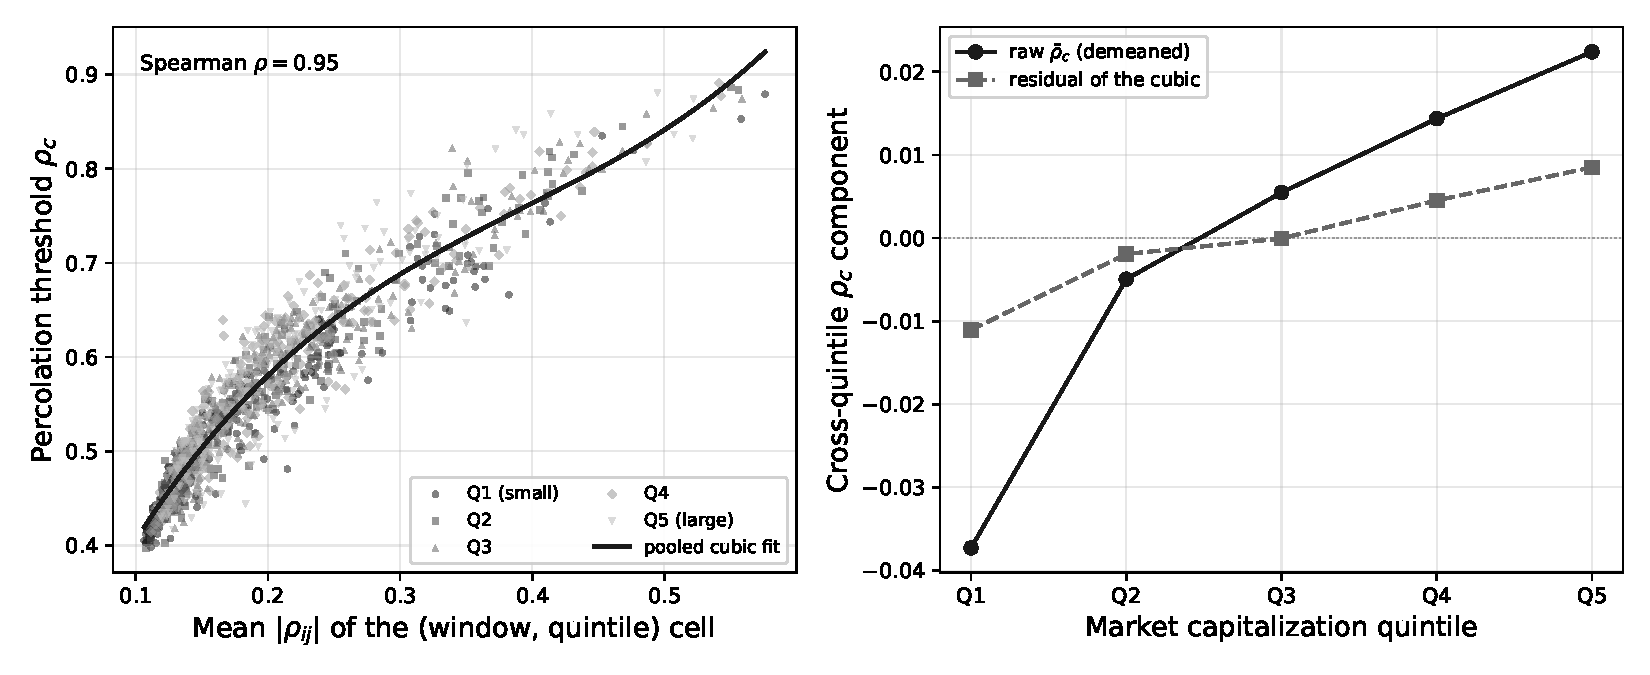
\includegraphics[width=0.95\textwidth]{../figures/fig_rho_c_vs_mean.pdf}
\caption{Percolation threshold and mean correlation, Korea. Left: $\rho_c$ against the mean $|\rho_{ij}|$ of the same (window, quintile) cell, one marker style per quintile, with the cubic fitted over all cells (solid line) and the Spearman rank correlation over all cells. Right: the demeaned quintile means of $\rho_c$ and the quintile means of the residuals of the cubic. Both rise from Q1 to Q5, the residuals by \rhoCResidGapPctOfRaw\ of the rise of $\rho_c$.}\label{fig:si_rho_c_vs_mean}
\end{figure}

% ============================================================
% S.4 SIMULATION OF THE MODEL
% ============================================================
\section{The Derivative of the Return Variance}\label{si:variance_derivative}

Each variance of main-paper Eq.~\eqref{eq:toy_var} has the derivative $2\sigma_u^2[\delta - (1-\delta)\sum_k W_{ik}^2]$ in $\delta$. The entries of $W$ lie in $[0,1]$ and its row sums are at most one, so $\sum_k W_{ik}^2 \leq 1$. For $\delta \geq 1/2$, therefore, $\delta \geq 1-\delta \geq (1-\delta)\sum_k W_{ik}^2$, so the derivative is non-negative and each variance rises with $\delta$ on $[1/2, 1)$.

\section{Simulation of the Return-Generating Model}\label{si:dgp_validation}

The simulation draws returns from main-paper Eq.~\eqref{eq:toy_rgp} and passes them to the estimation of the main paper, which gives the simulated threshold $\rho_c^{\mathrm{sim}}$. It uses $T = \dgpT$ trading days, $N = \dgpN$ stocks per segment, the idiosyncratic standard deviation $\sigma_u = \dgpSigmaU$, and the values of $\delta$ from $\dgpDeltaGridMin$ to $\dgpDeltaGridMax$ that Table~\ref{tab:dgp_eq9} lists. It uses two peer-coupling matrices, each scaled to unit row sums. The first links each stock to $k = \dgpKnnK$ others at random, and the second groups the stocks into \dgpNSectors\ sectors with weight \dgpIntraWeight\ within a sector and \dgpInterWeight\ between sectors. The loadings are drawn with fixed seeds from a normal distribution with mean \dgpBetaMean\ and standard deviation \dgpBetaStd, clipped to $[\dgpBetaLo, \dgpBetaHi]$ so that all loadings share a sign. The factor standard deviation $\sigma_f = \dgpSigmaF$ is \dgpSigmaFScale\ times \dgpSigmaFUnscaled, a round value for the daily standard deviation of a market index's return. The multiplier is set from data so that the simulated $\rho_c$ over the grid of $\delta$ brackets the range of the Korean cross-window means, from \barRhoCQone\ to \barRhoCQfive, whereas the sign prediction of the main paper for $\delta \geq 1/2$ is analytic and uses no parameter set from data.

\label{si:eq9_verification}Table~\ref{tab:dgp_eq9} gives the simulated threshold $\rho_c^{\mathrm{sim}}$, the model's threshold $\tilde\rho_c$ of main-paper Eq.~\eqref{eq:toy_threshold}, and the closed form in each of the \nDgpEqEightCells\ cells of $\delta$ and peer-coupling matrix. The closed form of main-paper Eq.~\eqref{eq:toy_closed_form} orders the values of $\delta$ as $\rho_c^{\mathrm{sim}}$ does but lies above $\rho_c^{\mathrm{sim}}$ by \dgpEqNineOvershootLo\ to \dgpEqNineOvershootHi, because it keeps only the leading-order root of main-paper Eq.~\eqref{eq:toy_gauss}, which lies above the exact normal quantile, and because the upper tail of the simulated correlations is not normal. The closed form therefore predicts the direction of the dependence on $\delta$ but not the level of $\rho_c$.

\begin{table}[pos=htbp]
\centering
\begin{threeparttable}
\caption{Simulated threshold, random-graph criterion, and closed form, by $\delta$ and peer-coupling matrix.}\label{tab:dgp_eq9}
\begin{tabular}{ccccc}
\toprule
$\delta$ & Matrix & $\rho_c^{\mathrm{sim}}$ & $\tilde\rho_c$ & Closed form \\
\midrule
0.40 & random & \rhoCDgpSimDeltaA       & \rhoCDgpSimDegOneDeltaA       & \rhoCDgpClosedDeltaA       \\
0.50 & random & \rhoCDgpSimDeltaB       & \rhoCDgpSimDegOneDeltaB       & \rhoCDgpClosedDeltaB       \\
0.60 & random & \rhoCDgpSimDeltaC       & \rhoCDgpSimDegOneDeltaC       & \rhoCDgpClosedDeltaC       \\
0.70 & random & \rhoCDgpSimDeltaD       & \rhoCDgpSimDegOneDeltaD       & \rhoCDgpClosedDeltaD       \\
0.85 & random & \rhoCDgpSimDeltaE       & \rhoCDgpSimDegOneDeltaE       & \rhoCDgpClosedDeltaE       \\
0.40 & sector & \rhoCDgpSimSectorDeltaA & \rhoCDgpSimSectorDegOneDeltaA & \rhoCDgpClosedSectorDeltaA \\
0.50 & sector & \rhoCDgpSimSectorDeltaB & \rhoCDgpSimSectorDegOneDeltaB & \rhoCDgpClosedSectorDeltaB \\
0.60 & sector & \rhoCDgpSimSectorDeltaC & \rhoCDgpSimSectorDegOneDeltaC & \rhoCDgpClosedSectorDeltaC \\
0.70 & sector & \rhoCDgpSimSectorDeltaD & \rhoCDgpSimSectorDegOneDeltaD & \rhoCDgpClosedSectorDeltaD \\
0.85 & sector & \rhoCDgpSimSectorDeltaE & \rhoCDgpSimSectorDegOneDeltaE & \rhoCDgpClosedSectorDeltaE \\
\bottomrule
\end{tabular}
\begin{tablenotes}
\small
\item \textit{Notes:} \dgpEqNineNMc\ replicates per cell, each with its own draw of the matrix and the loadings. $\rho_c^{\mathrm{sim}}$ is the cutoff of fastest change of $G$, estimated as in the main paper. $\tilde\rho_c$ is the quantile $1 - 1/(N-1)$ of the simulated $|\rho_{ij}|$, the threshold of main-paper Eq.~\eqref{eq:toy_threshold}. The closed form is main-paper Eq.~\eqref{eq:toy_closed_form}. ``Random'' links each stock to \dgpKnnK\ others at random, and ``sector'' couples stocks within and between \dgpNSectors\ sectors.
\end{tablenotes}
\end{threeparttable}
\end{table}

% ============================================================
% REFERENCES
% ============================================================
\bibliographystyle{elsarticle-num-names}
\bibliography{references}

\end{document}
